\documentclass[a4paper,12pt]{article}
\usepackage[utf8]{inputenc}
\usepackage[polish]{babel}
\usepackage{graphicx}
\usepackage{geometry}
\usepackage{hyperref}
\usepackage{float}
\geometry{margin=2.5cm}

\title{Podsumowanie eksperymentów numerycznych\thanks{Automatycznie wygenerowano -- {\today}}}
\author{Autor: Greg}
\date{\today}

\begin{document}
\maketitle
\tableofcontents
\newpage

\section{Wstęp}
Celem niniejszego raportu jest podsumowanie wyników eksperymentów numerycznych przeprowadzonych dla trzech funkcji testowych: kwadratowej, Rosenbrocka oraz Ackleya, w wymiarach $n=10$ oraz $n=30$. Analizowano wpływ parametrów $\sigma$ oraz $a$ na przebieg optymalizacji. Wyniki przedstawiono w postaci wykresów median wartości funkcji celu oraz parametru $\sigma$ w czasie.

\section{Opis eksperymentów}
Dla każdej funkcji i wymiaru przeprowadzono eksperymenty dla kombinacji $\sigma \in \{0.1, 1.0, 10.0\}$ oraz $a \in \{10, 100\}$. Każda konfiguracja była powtarzana 10 razy. Na wykresach zbiorczych przedstawiono mediany przebiegów dla wszystkich kombinacji parametrów.

% --- Quadratic n=10 ---
\section{Funkcja kwadratowa, $n=10$}
\subsection{Mediana wartości funkcji celu}
\begin{figure}[H]
    \centering
    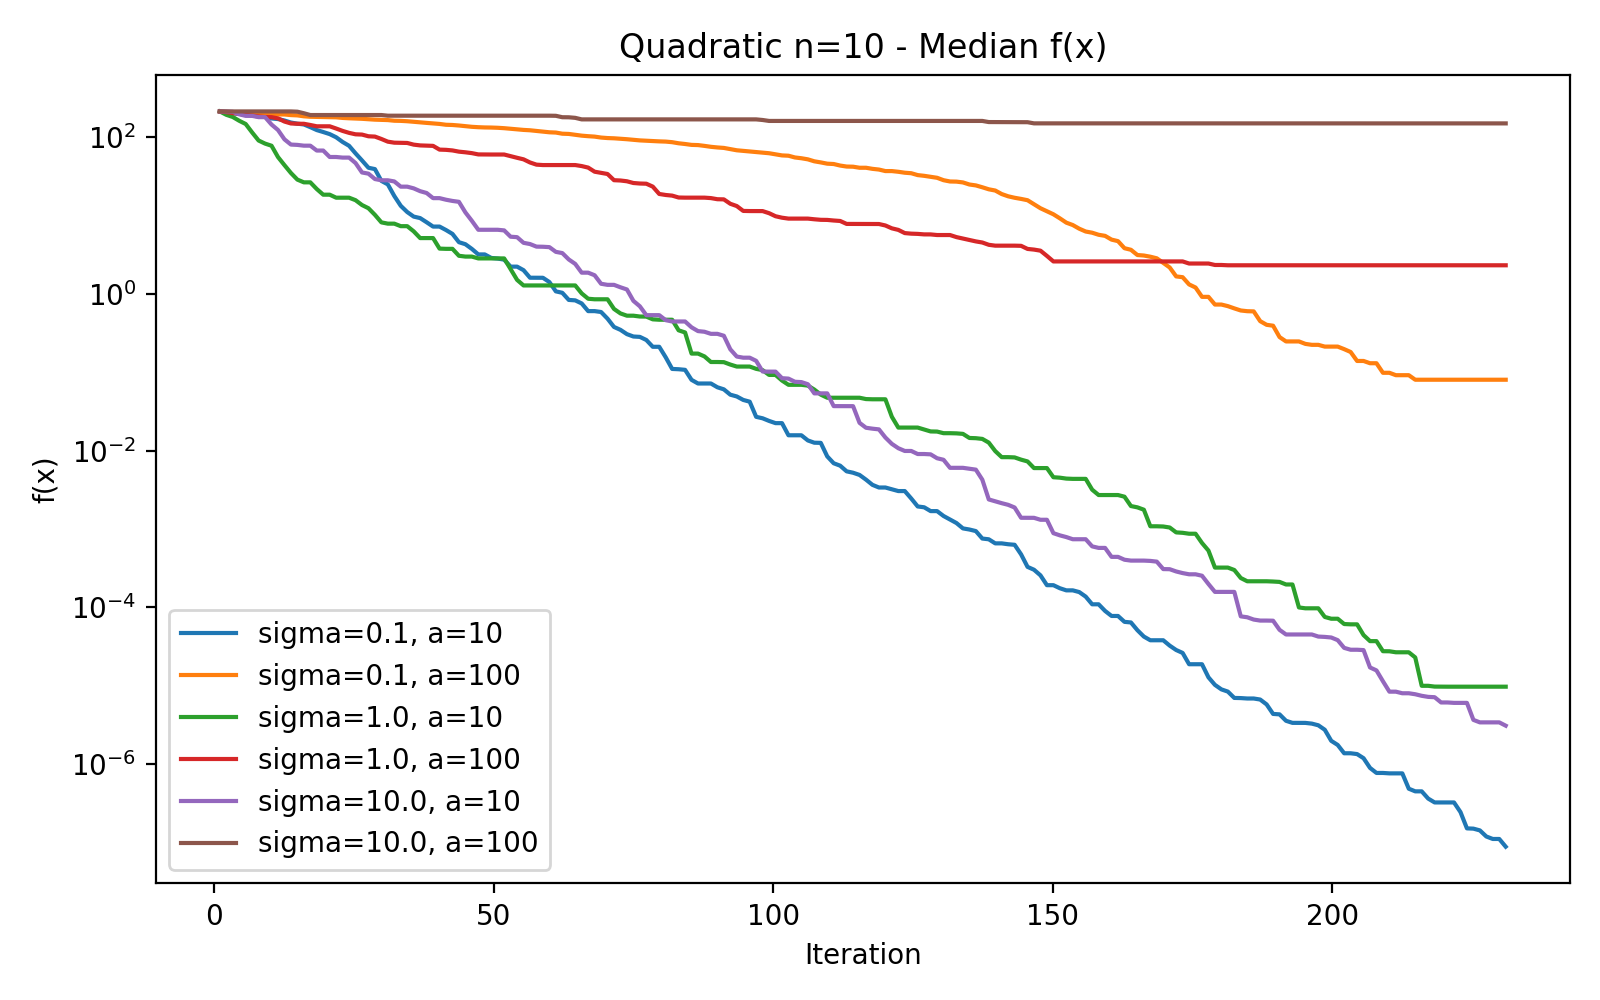
\includegraphics[width=0.8\textwidth]{charts/Quadratic_n10_all_medians.png}
    \caption{Mediany $f(t)$ dla funkcji kwadratowej ($n=10$) dla różnych $\sigma$ i $a$.}
\end{figure}
\subsection{Mediana $\sigma(t)$}
\begin{figure}[H]
    \centering
    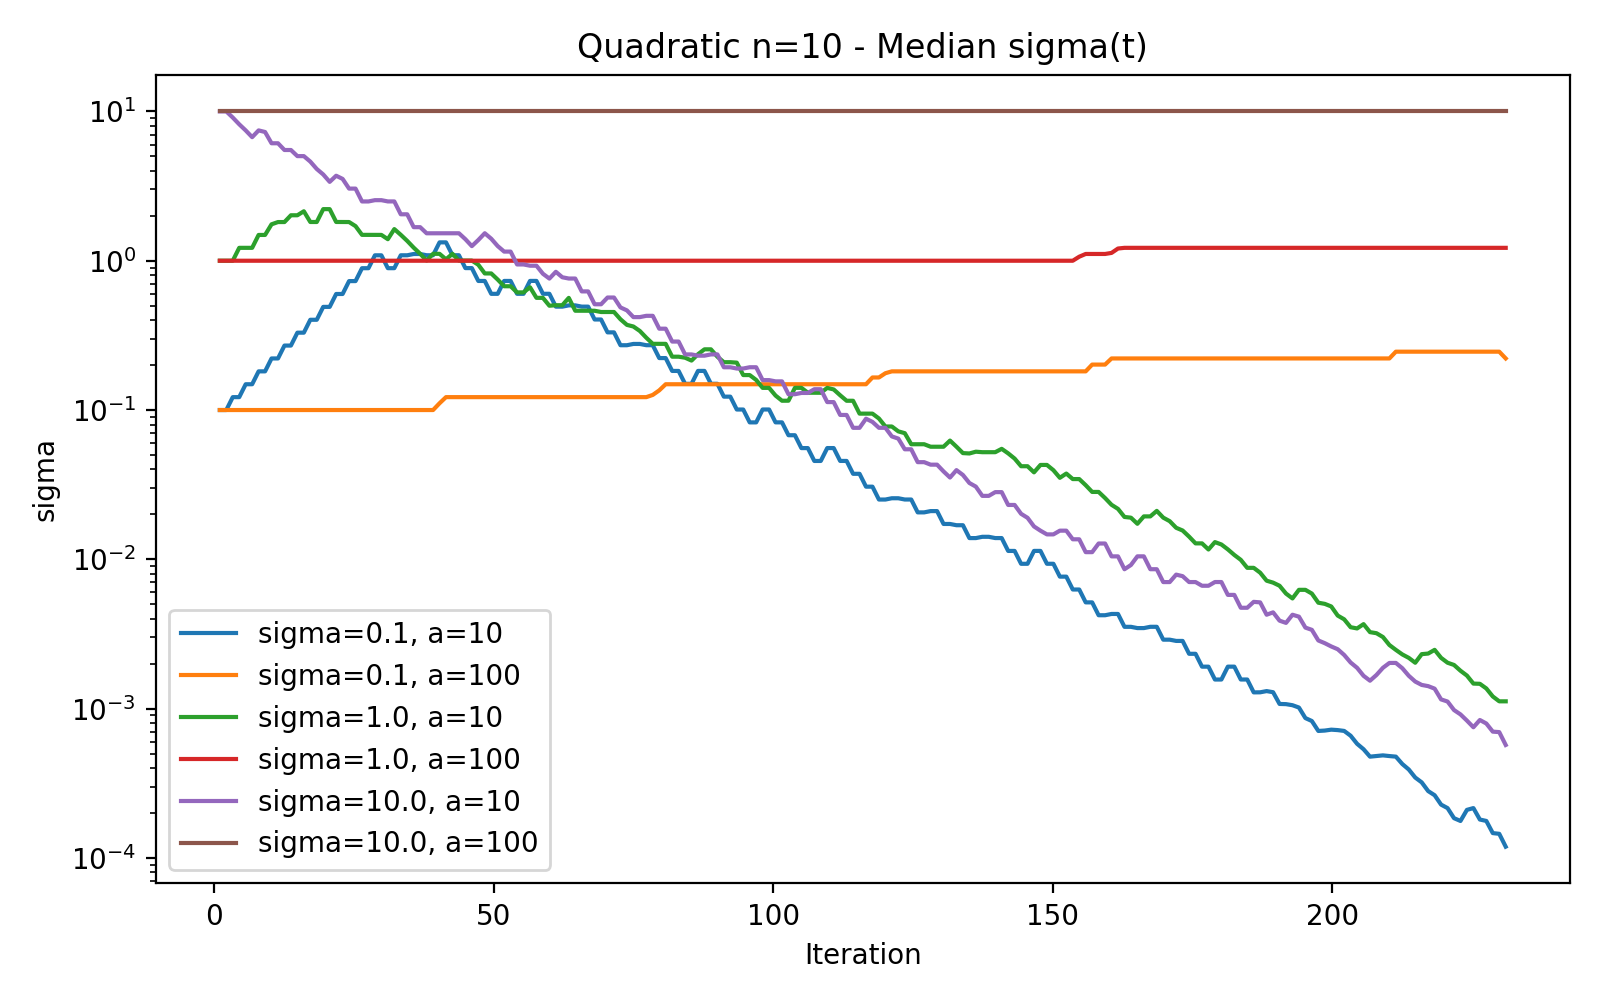
\includegraphics[width=0.8\textwidth]{charts/Quadratic_n10_all_sigmas.png}
    \caption{Mediany $\sigma(t)$ dla funkcji kwadratowej ($n=10$) dla różnych $\sigma$ i $a$.}
\end{figure}

% --- Quadratic n=30 ---
\section{Funkcja kwadratowa, $n=30$}
\subsection{Mediana wartości funkcji celu}
\begin{figure}[H]
    \centering
    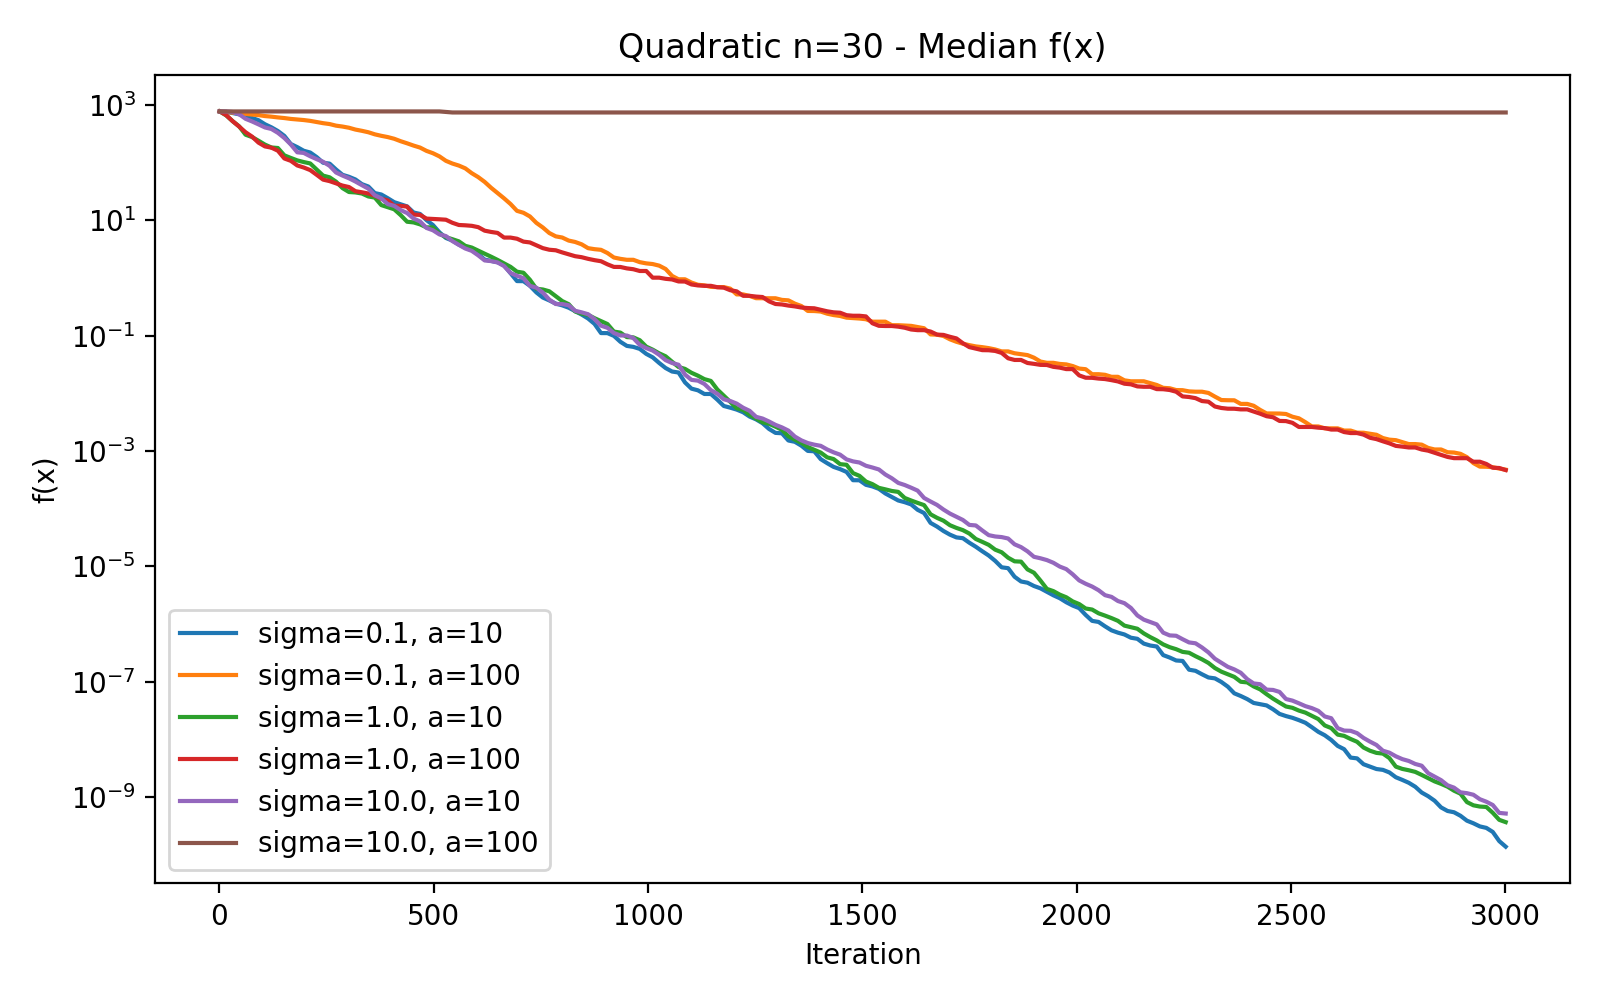
\includegraphics[width=0.8\textwidth]{charts/Quadratic_n30_all_medians.png}
    \caption{Mediany $f(t)$ dla funkcji kwadratowej ($n=30$) dla różnych $\sigma$ i $a$.}
\end{figure}
\subsection{Mediana $\sigma(t)$}
\begin{figure}[H]
    \centering
    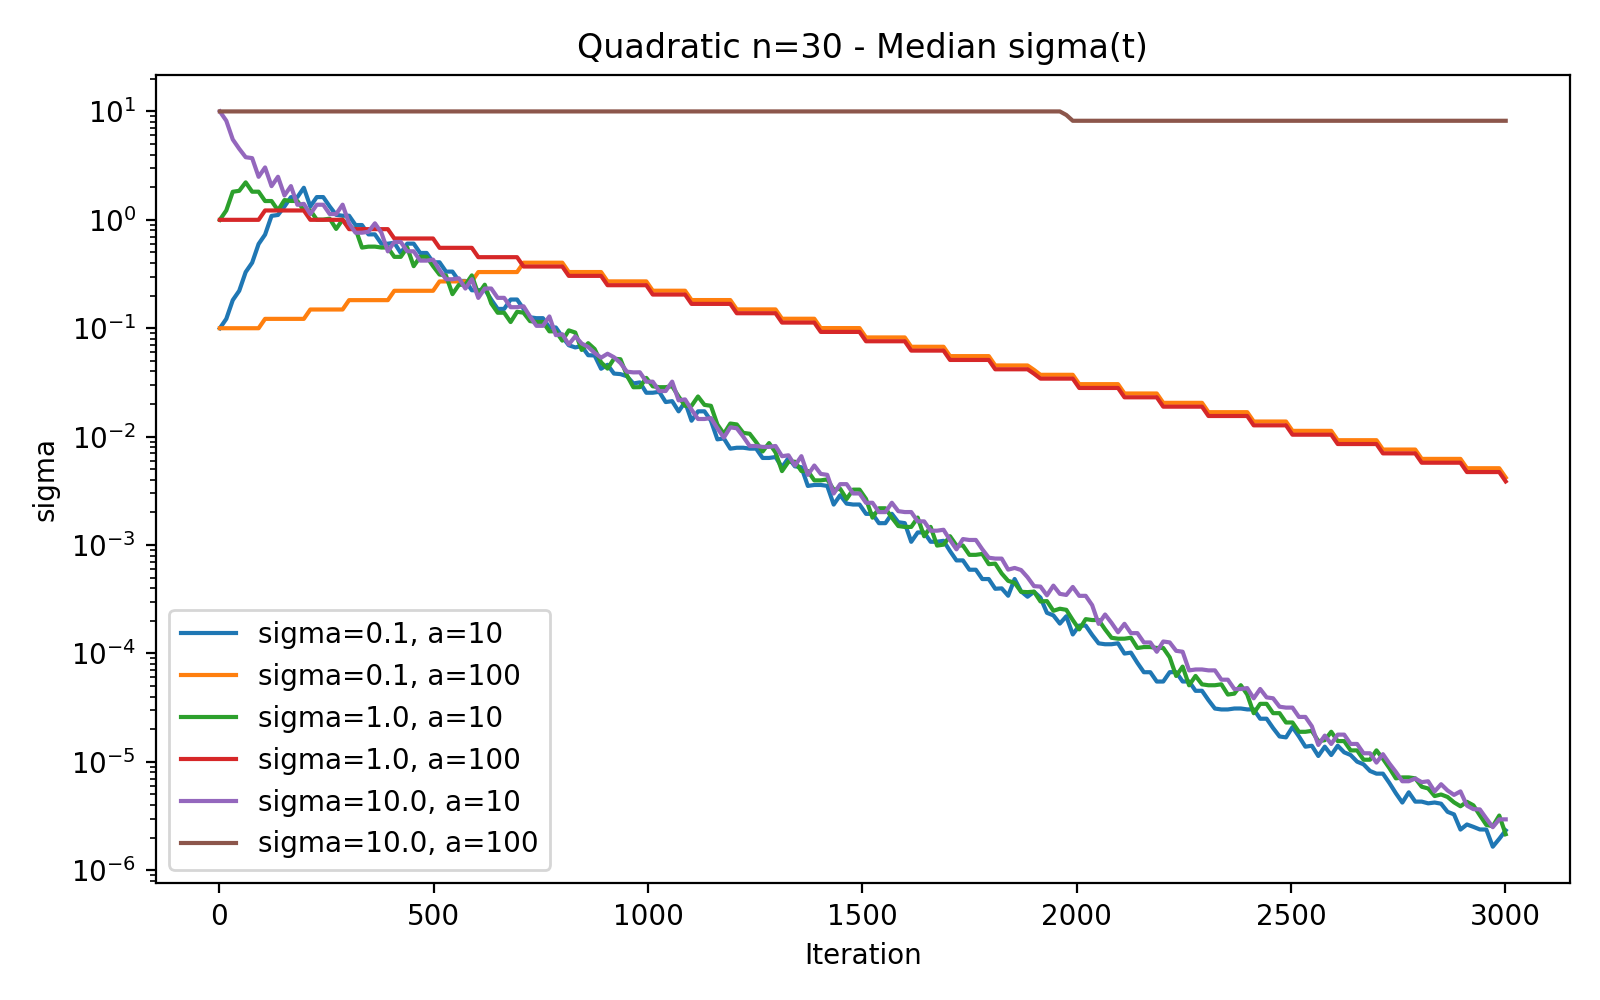
\includegraphics[width=0.8\textwidth]{charts/Quadratic_n30_all_sigmas.png}
    \caption{Mediany $\sigma(t)$ dla funkcji kwadratowej ($n=30$) dla różnych $\sigma$ i $a$.}
\end{figure}

% --- Rosenbrock n=10 ---
\section{Funkcja Rosenbrocka, $n=10$}
\subsection{Mediana wartości funkcji celu}
\begin{figure}[H]
    \centering
    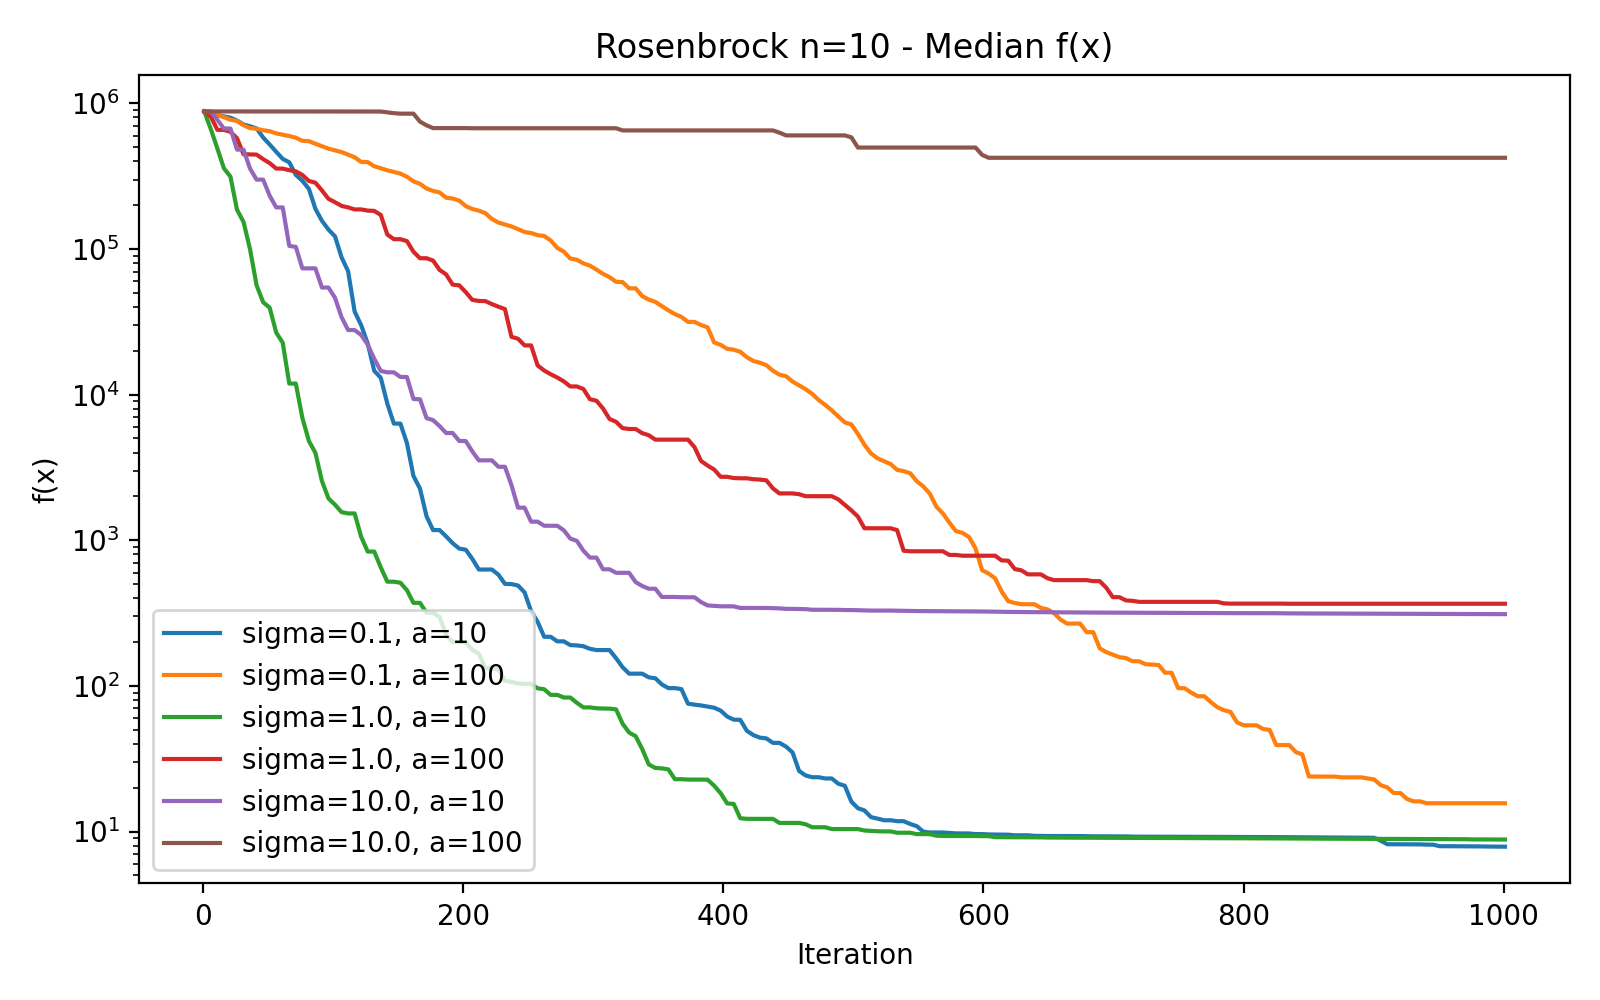
\includegraphics[width=0.8\textwidth]{charts/Rosenbrock_n10_all_medians.png}
    \caption{Mediany $f(t)$ dla funkcji Rosenbrocka ($n=10$) dla różnych $\sigma$ i $a$.}
\end{figure}
\subsection{Mediana $\sigma(t)$}
\begin{figure}[H]
    \centering
    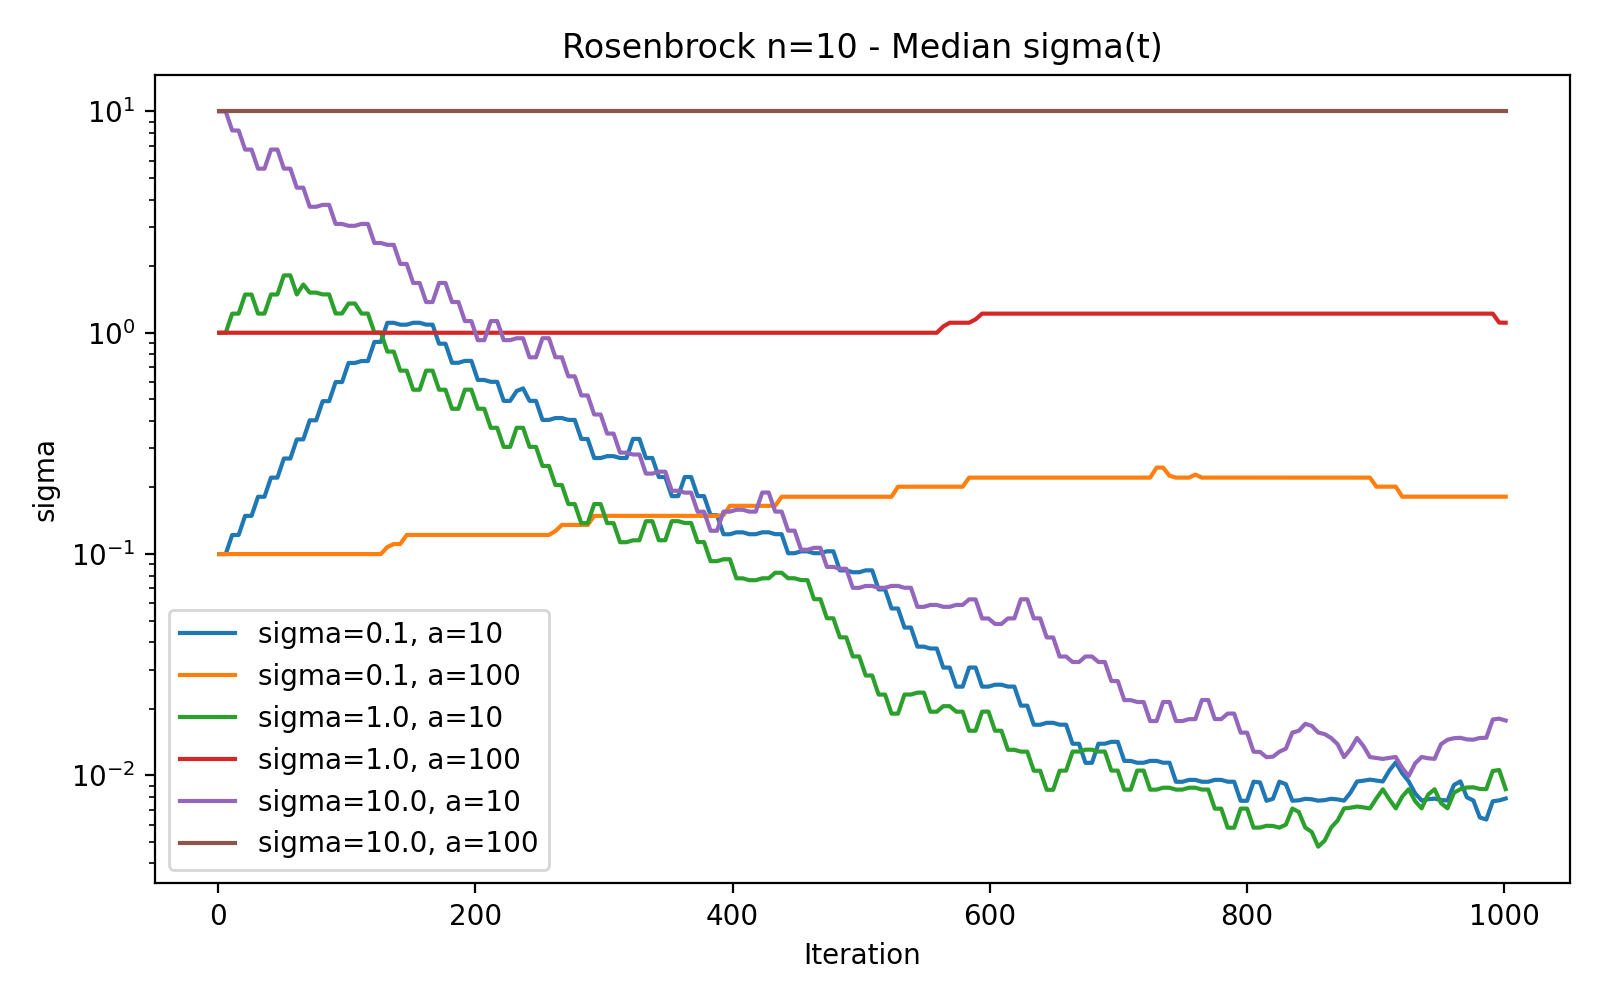
\includegraphics[width=0.8\textwidth]{charts/Rosenbrock_n10_all_sigmas.png}
    \caption{Mediany $\sigma(t)$ dla funkcji Rosenbrocka ($n=10$) dla różnych $\sigma$ i $a$.}
\end{figure}

% --- Rosenbrock n=30 ---
\section{Funkcja Rosenbrocka, $n=30$}
\subsection{Mediana wartości funkcji celu}
\begin{figure}[H]
    \centering
    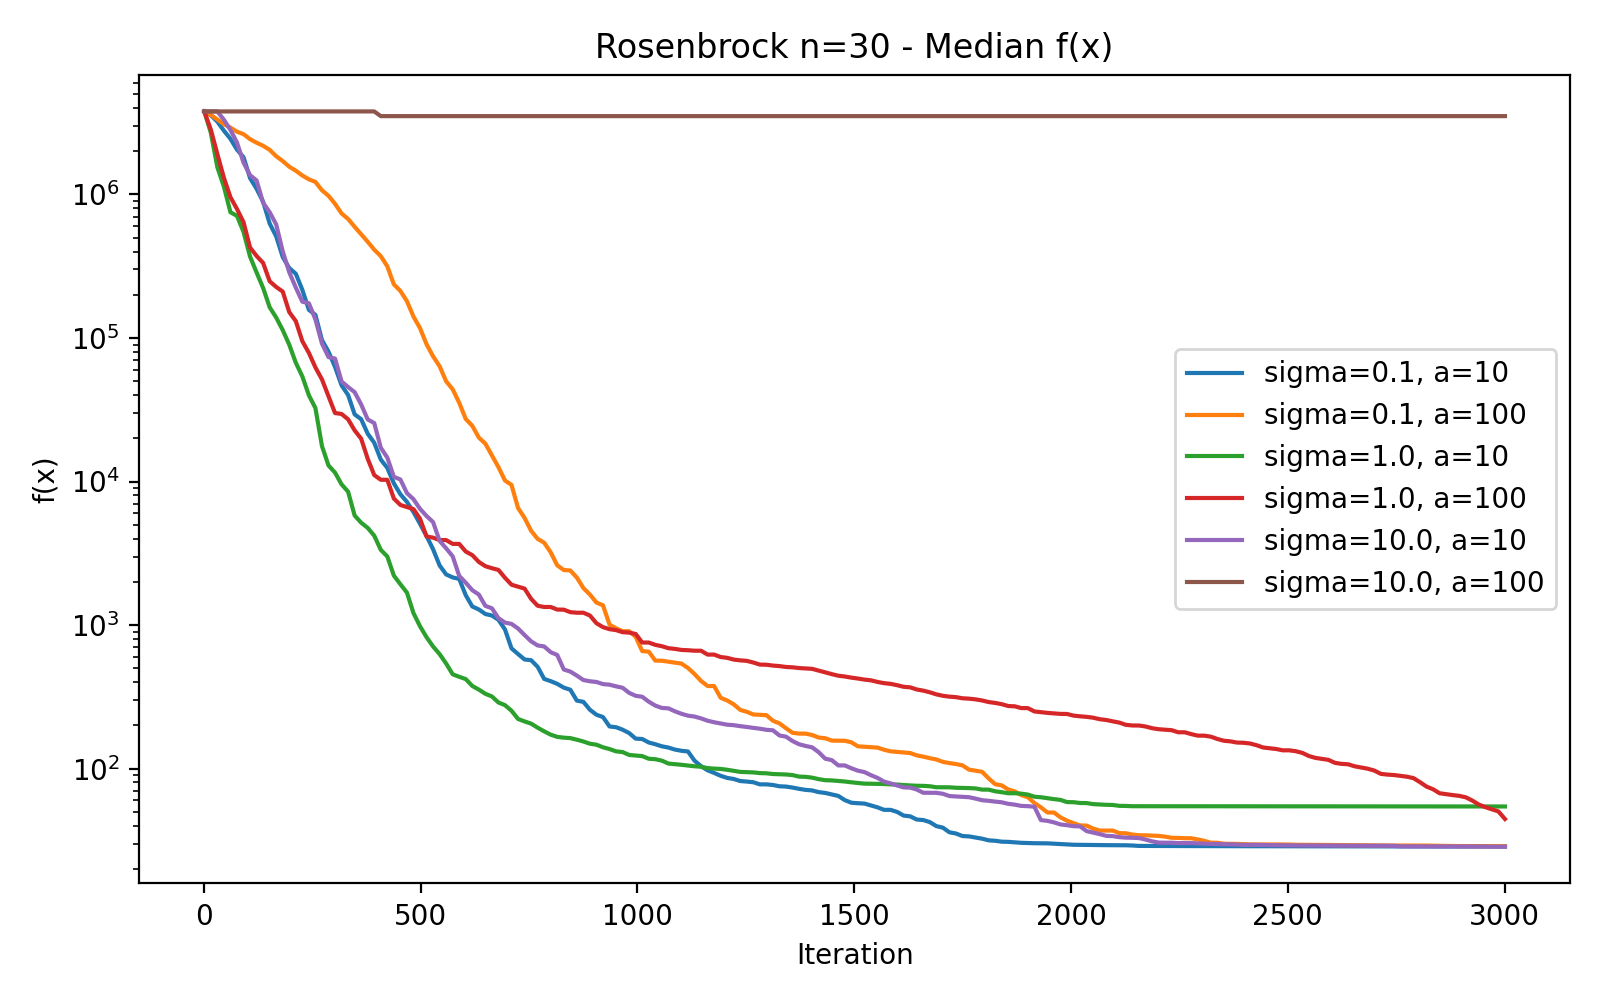
\includegraphics[width=0.8\textwidth]{charts/Rosenbrock_n30_all_medians.png}
    \caption{Mediany $f(t)$ dla funkcji Rosenbrocka ($n=30$) dla różnych $\sigma$ i $a$.}
\end{figure}
\subsection{Mediana $\sigma(t)$}
\begin{figure}[H]
    \centering
    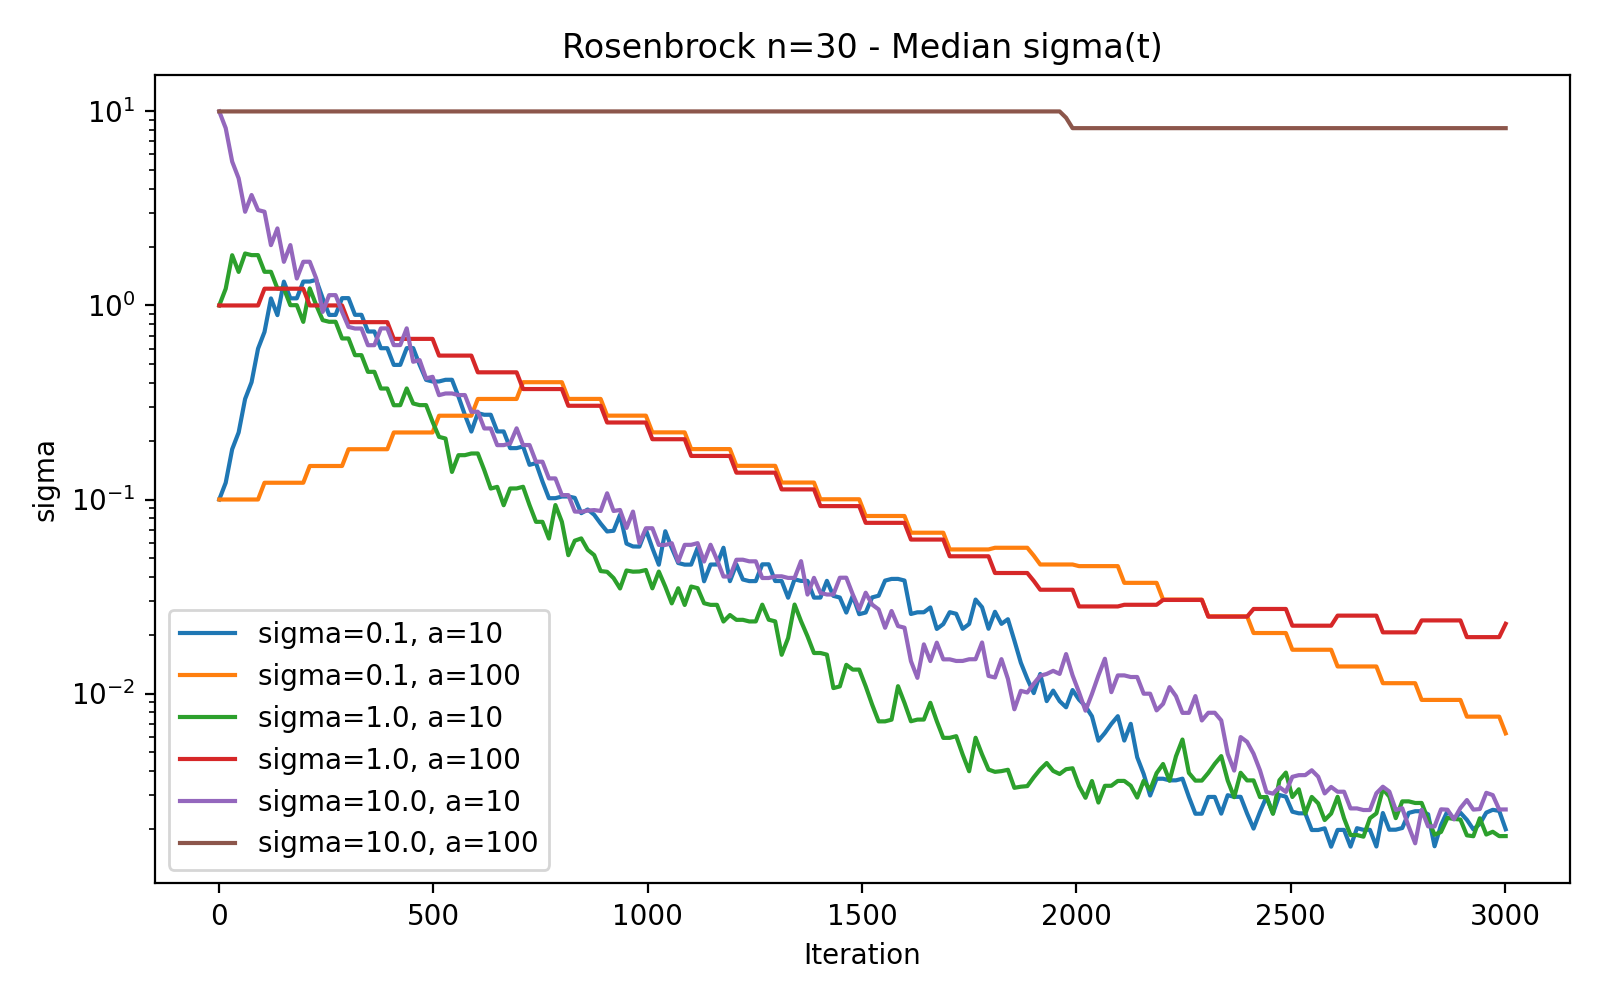
\includegraphics[width=0.8\textwidth]{charts/Rosenbrock_n30_all_sigmas.png}
    \caption{Mediany $\sigma(t)$ dla funkcji Rosenbrocka ($n=30$) dla różnych $\sigma$ i $a$.}
\end{figure}

% --- Ackley n=10 ---
\section{Funkcja Ackleya, $n=10$}
\subsection{Mediana wartości funkcji celu}
\begin{figure}[H]
    \centering
    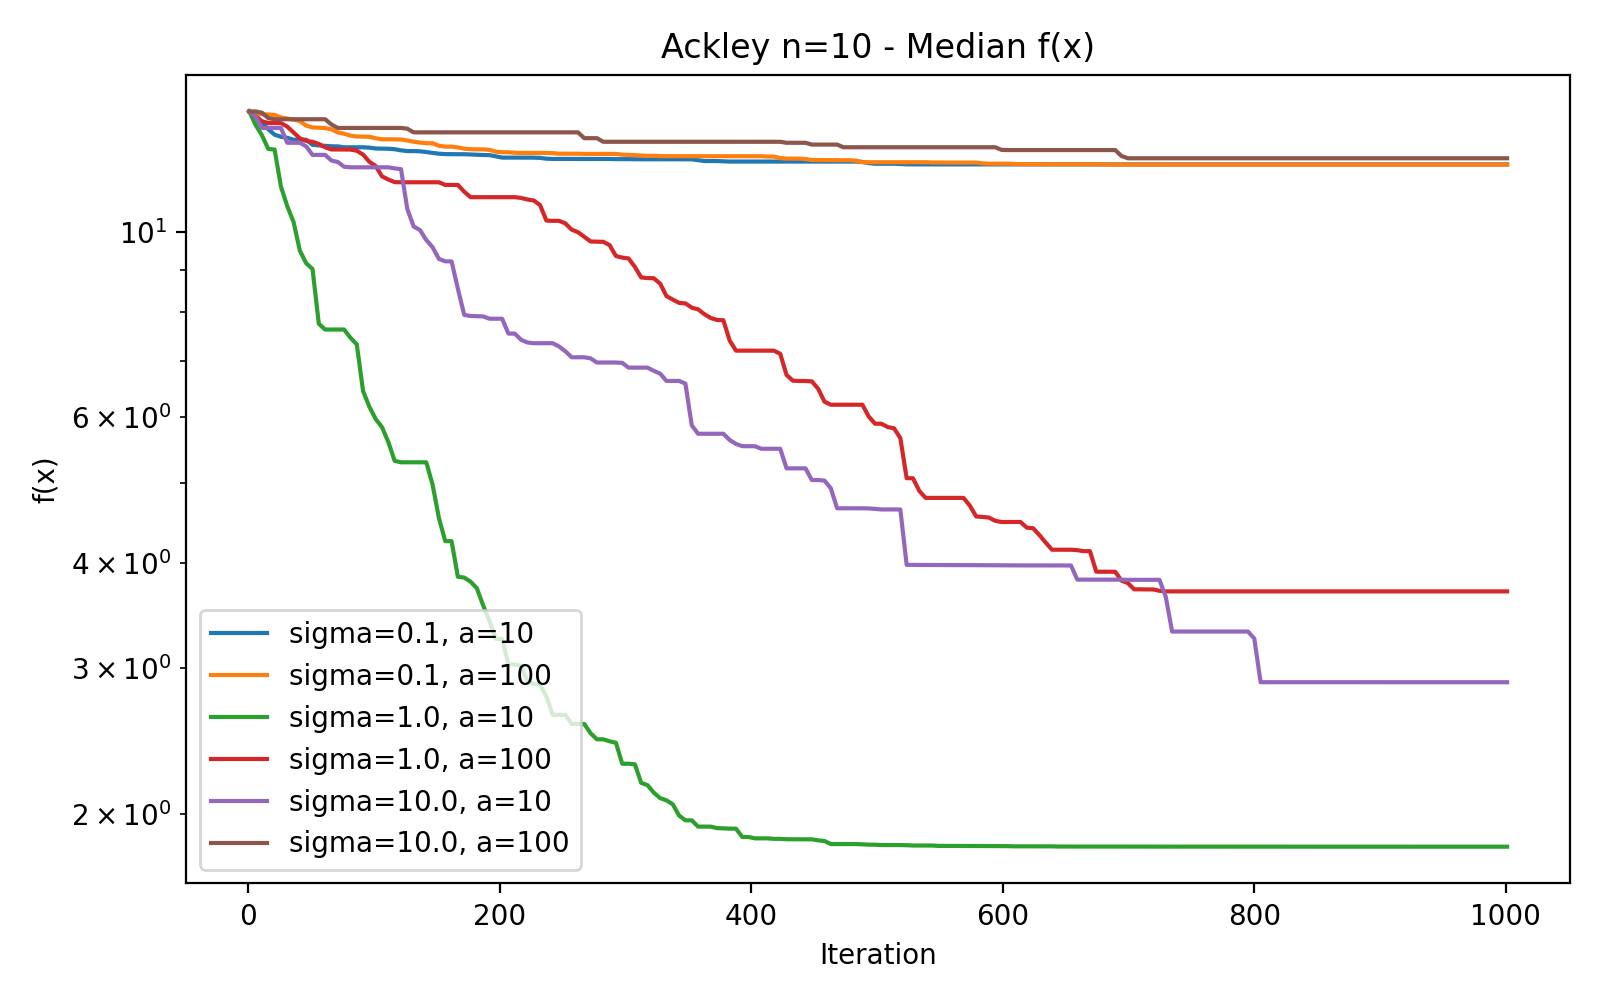
\includegraphics[width=0.8\textwidth]{charts/Ackley_n10_all_medians.png}
    \caption{Mediany $f(t)$ dla funkcji Ackleya ($n=10$) dla różnych $\sigma$ i $a$.}
\end{figure}
\subsection{Mediana $\sigma(t)$}
\begin{figure}[H]
    \centering
    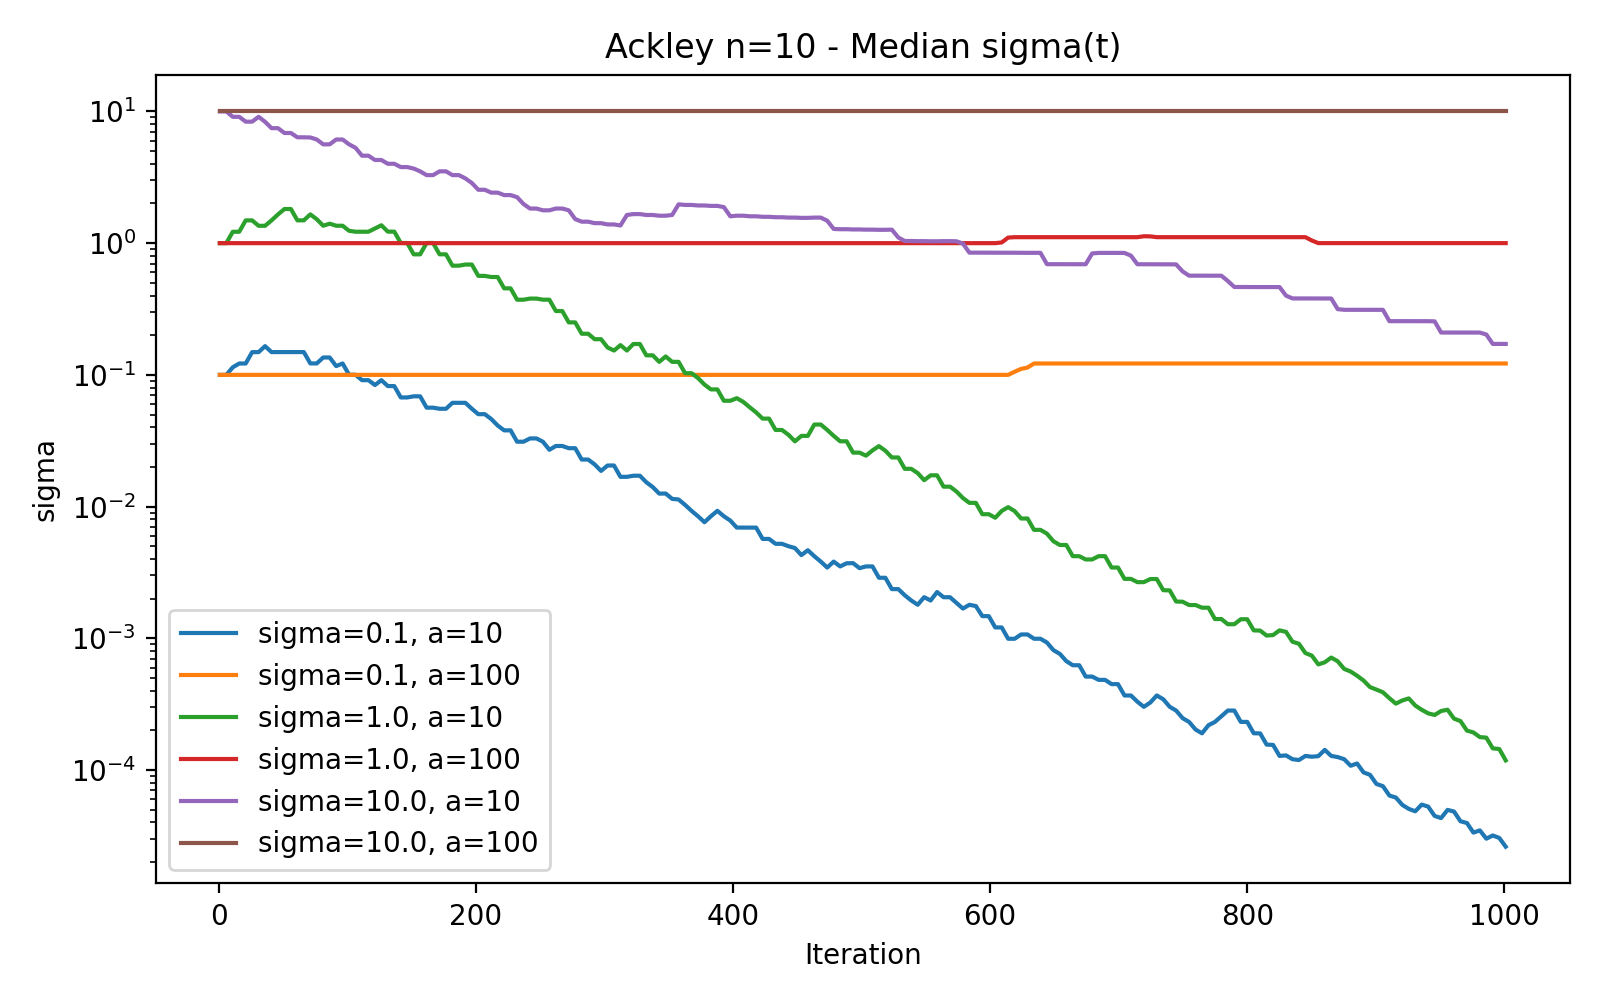
\includegraphics[width=0.8\textwidth]{charts/Ackley_n10_all_sigmas.png}
    \caption{Mediany $\sigma(t)$ dla funkcji Ackleya ($n=10$) dla różnych $\sigma$ i $a$.}
\end{figure}

% --- Ackley n=30 ---
\section{Funkcja Ackleya, $n=30$}
\subsection{Mediana wartości funkcji celu}
\begin{figure}[H]
    \centering
    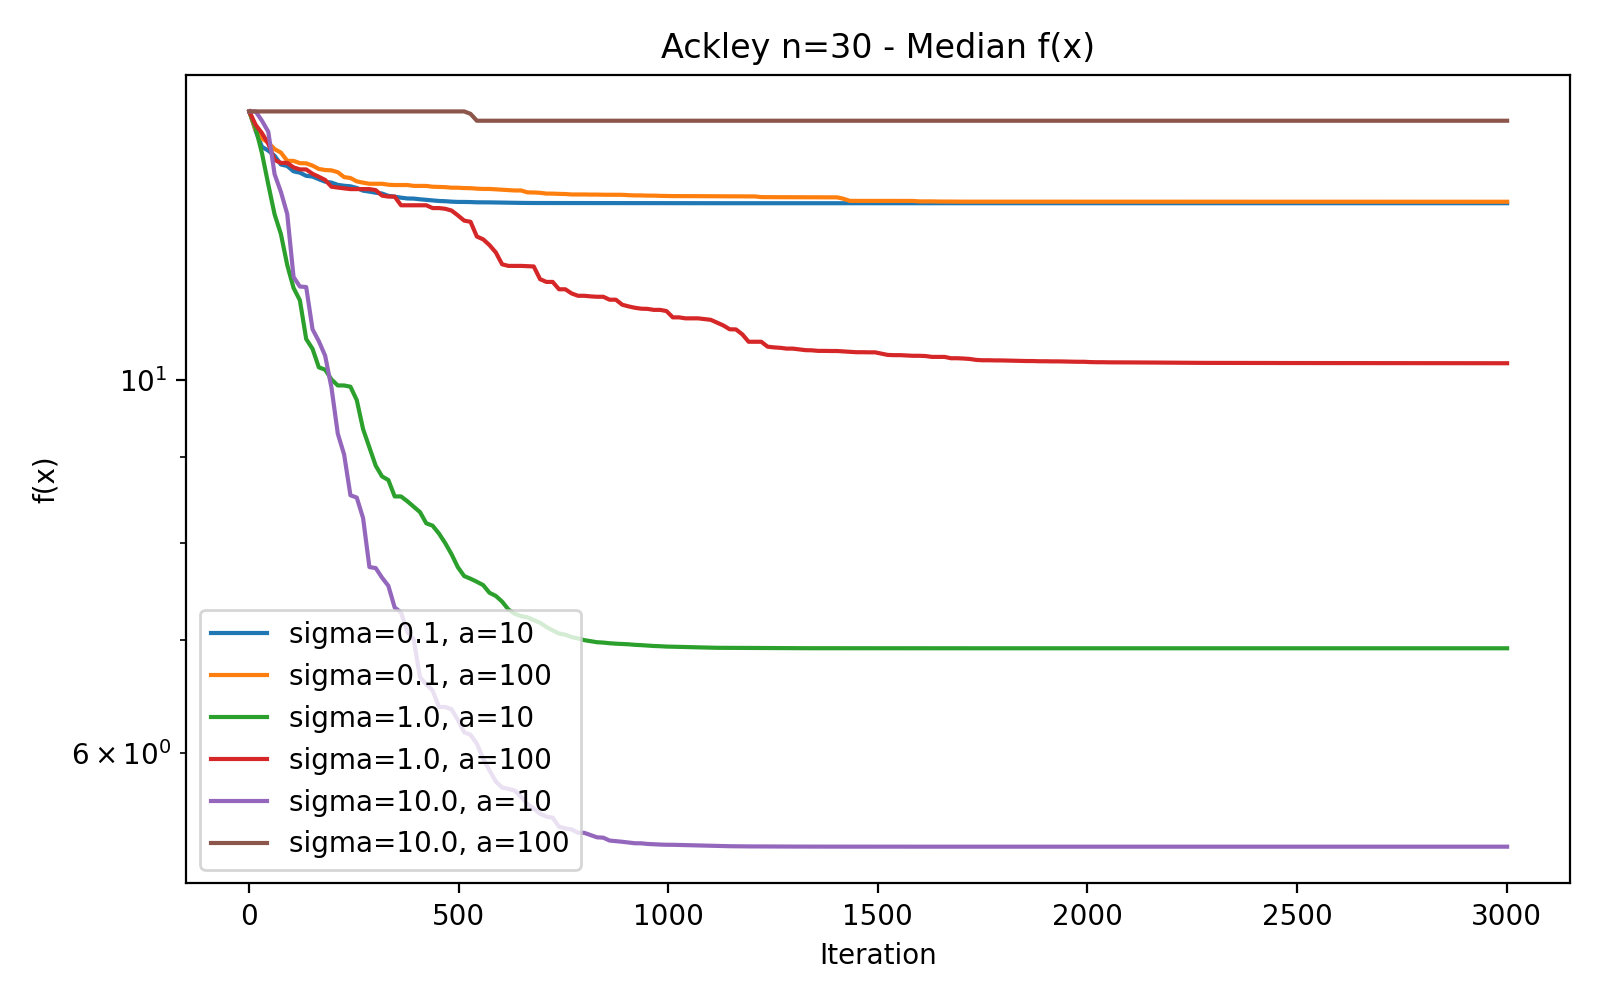
\includegraphics[width=0.8\textwidth]{charts/Ackley_n30_all_medians.png}
    \caption{Mediany $f(t)$ dla funkcji Ackleya ($n=30$) dla różnych $\sigma$ i $a$.}
\end{figure}
\subsection{Mediana $\sigma(t)$}
\begin{figure}[H]
    \centering
    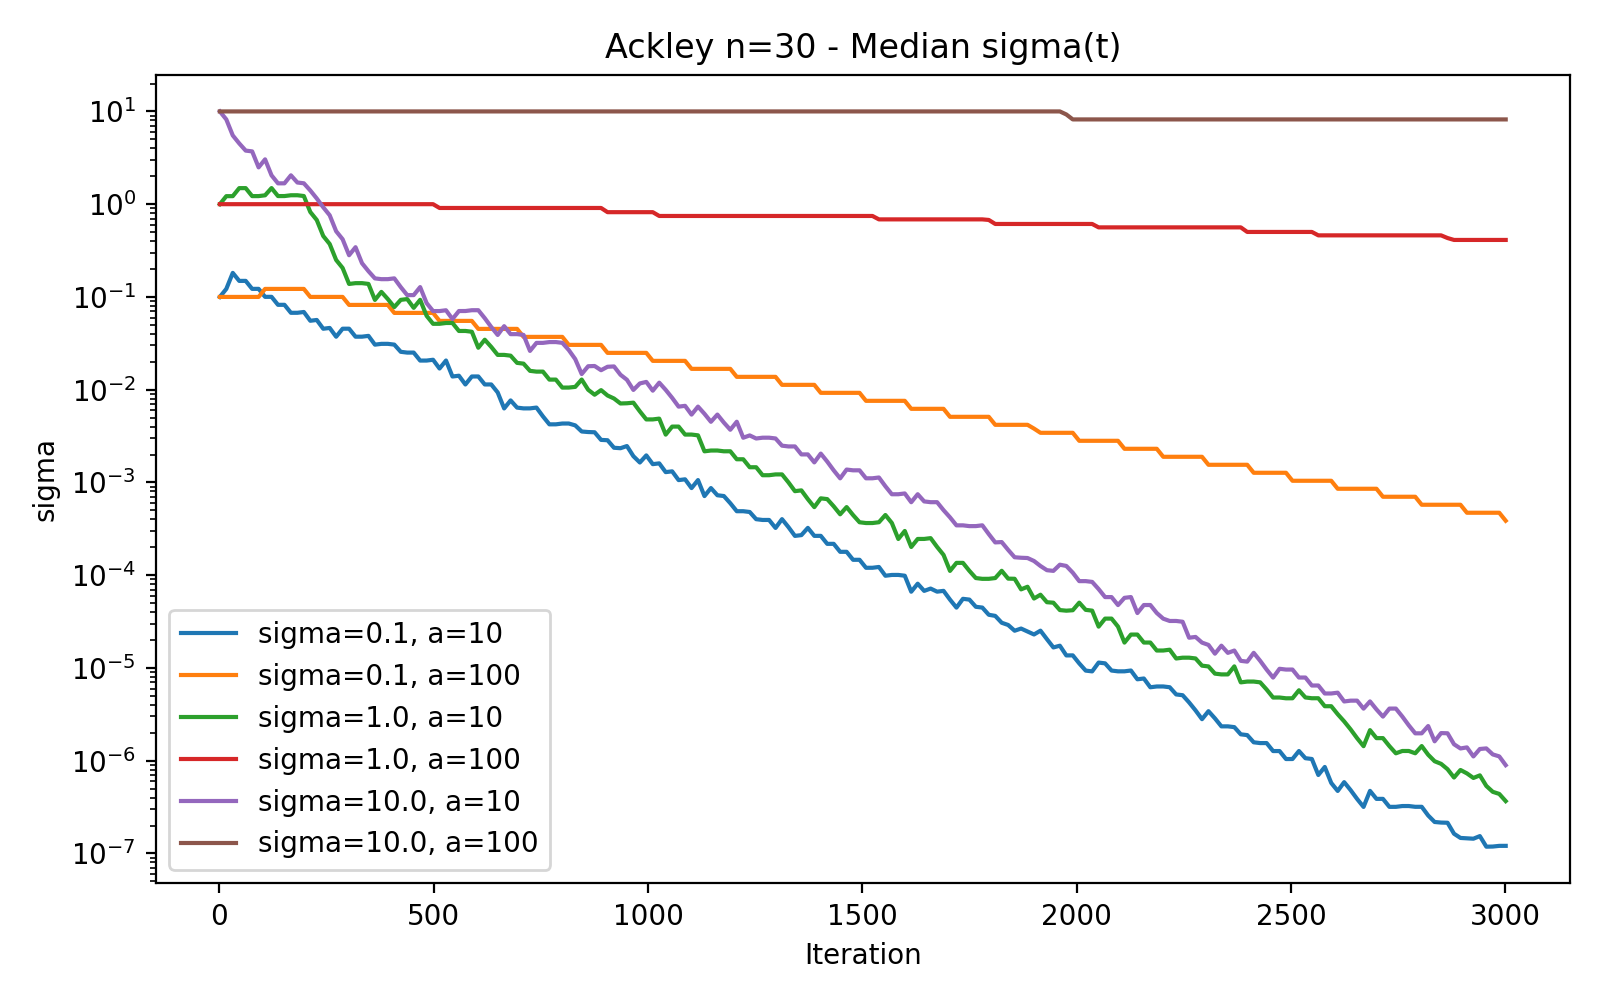
\includegraphics[width=0.8\textwidth]{charts/Ackley_n30_all_sigmas.png}
    \caption{Mediany $\sigma(t)$ dla funkcji Ackleya ($n=30$) dla różnych $\sigma$ i $a$.}
\end{figure}

\newpage
\section{Podsumowanie}
Przeprowadzone eksperymenty pozwalają na analizę wpływu parametrów $\sigma$ i $a$ na efektywność optymalizacji. Wartości median $f(t)$ oraz $\sigma(t)$ umożliwiają porównanie stabilności i szybkości zbieżności algorytmu dla różnych ustawień. Szczegółowe wnioski można wyciągnąć na podstawie kształtu i przebiegu wykresów.

\end{document}
